\chapter{\label{chap:modeling}Modelagem do Sistema}

Conforme visto final do \ref{chap:simulation}, um sistema de simulação possui
uma série responsabilidades bem definidas. Neste estudo o sistema será projetado
através das construções do paradigma da orientação à objetos. A opção pela
Orientação à Objetos se dá por diversos motivos:

\begin{itemize}
  \item encapsulamento
  \item abstração
  \item padrão de mercado
  \item padrão acadêmico
\end{itemize}

\section{Eventos e Tipos de Eventos}

O simulador é orientado à eventos. Logo, é necessário ter uma representação de
um evento na implementação. Um evento deve possuir as seguintes informações:
tipo de evento; horário em que o evento está agendado; um cliente (passageiro)
e/ou um elevador e/ou um andar do prédio\footnote{A existência de informações
sobre o cliente, o elevador e o andar dependem do tipo de evento.}. Já os tipos
de eventos possíveis são:

\begin{description}
  \item[Chegada de um cliente] um cliente chegou na fila de um andar;
  \item[Chegada de um elevador] um elevador chegou a um andar;
  \item[Elevador moveu-se para cima] um elevador moveu-se para cima;
  \item[Elevador moveu-se para baixo] um elevador moveu-se para baixo.
\end{description}

A figura \ref{fig:diagram:event} exibe o diagrama UML da classe \textit{Event} e
a enumeração \textit{EventType}.

\begin{figure}[htb!]
  \centering
  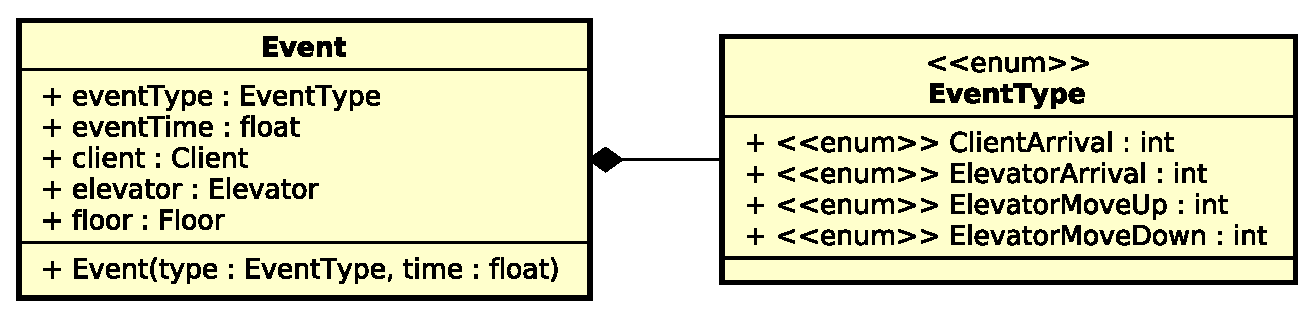
\includegraphics[scale=0.6]{img/event.eps}
  \caption{Classes para Eventos e Tipos de Eventos}
\label{fig:diagram:event}
\end{figure}

\section{Notificando Eventos}

Em um simulador, há a necessidade de executar diferentes ações na ocasião de um
evento específico. Por exemplo, atualizar o estado atual do sistema, as
estatísticas e o relógio da simulação. De acordo com Gamma
\cite{Gamma:1995:DPE:186897}, um \textit{design pattern} da programação
Orientada à Objetos indicado para o problema de notificar componentes que um
determinado evento ocorrereu é chamado de \textit{Observer}. Este
\textit{pattern} define uma dependência de um-para-muitos entre objetos de modo
que, quando este um objeto tem seu estado alterado, todos os seus dependentes
são notificados automaticamente. Por consequencia, estes objetos podem modificar
seu estado interno baseando-se nas informações desta notificação.

A figura \ref{fig:diagram:notification} ilustra as classes projetadas deste
sistema de Notificação de Eventos. A interface \textit{EventObserver} deve ser
realizada por qualquer classe que deseje receber eventos. Já a interface
\textit{EventNotifier} define a interface pública de um notificador de eventos.
Esta interface provê métodos que objetos \textit{EventObserver} possam se
registrar ou desregistrar para receber notificações das ocorrências de um
determinado tipo de evento, além de um método para realizar a notificação
propriamente dita do evento.

\begin{figure}[htb!]
  \centering
  \includegraphics[scale=0.6]{img/notification.eps}
  \caption{Diagrama de Classes do Notificador de Eventos}
\label{fig:diagram:notification}
\end{figure}

A classe concreta \textit{EventDispatcher} realiza a interface
\textit{EventNotifier}. Para armazenar os objetos que deverão receber
notificações para cada evento, é utilizado um mapa que relaciona tipo de evento
com uma lista de \textit{EventObservers}. Na ocasião da ocorrência de um evento,
o \textit{EventDispatcher} é responsável por varrer a sua lista interna de
assinantes e notificá-los conforme o tipo de evento ocorrido.

Esta construção é bastante útil no momento em que possuímos três importantes
componentes do sistema que necessitam alterar o seu estado interno a cada evento
ocorrido (figura \ref{fig:diagram:observers}). São eles: \textit{Timer},
responsável por encapsular o relógio da simulação; \textit{Statistics},
responsável pela acumulação das estatísticas da simulação; e \textit{Building},
entidade que armazena o estado do prédio em si, com seus andares, elevadores e
passageiros. Na ocorrência de um evento, estas três entidades devem ser
notificadas e cada uma irá alterar seu estado interno da forma que lhe convir.

\begin{figure}[htb!]
  \centering
  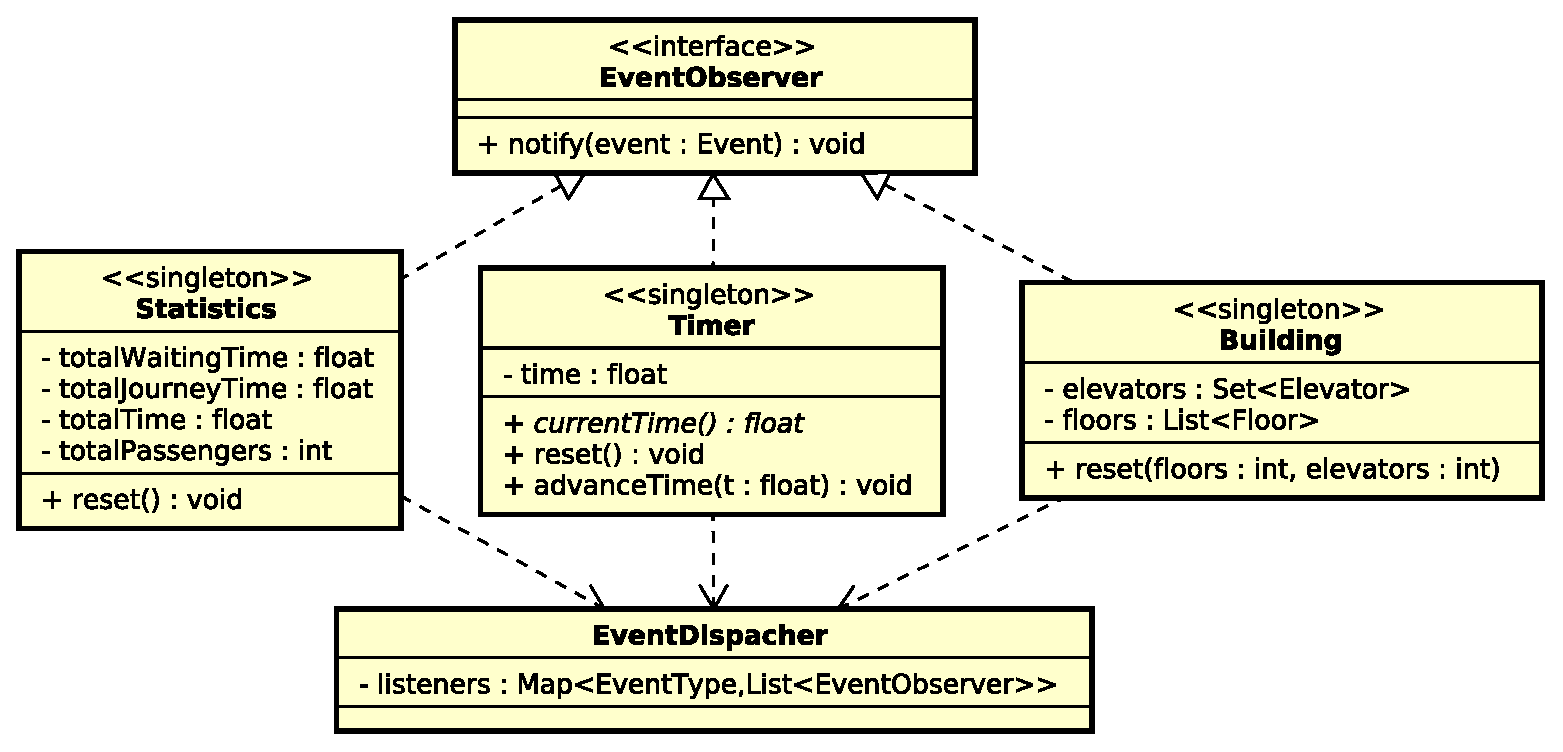
\includegraphics[scale=0.6]{img/observers.eps}
  \caption{Diagrama de Classes dos Observadores de Eventos}
\label{fig:diagram:observers}
\end{figure}

\begin{figure}[htb!]
  \centering
  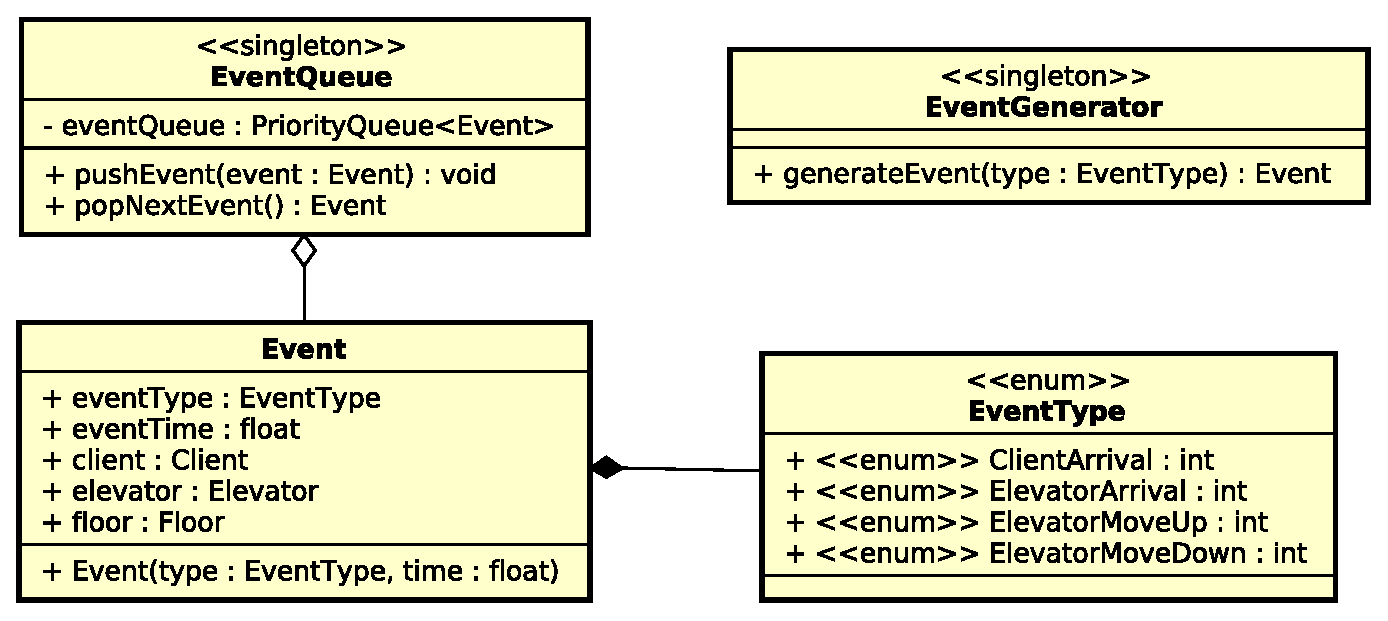
\includegraphics[scale=0.6]{img/event_management.eps}
  \caption{Diagrama de Classes do Gerenciador de Eventos}
\label{fig:diagram:event:manage}
\end{figure}

\begin{figure}[htb!]
  \centering
  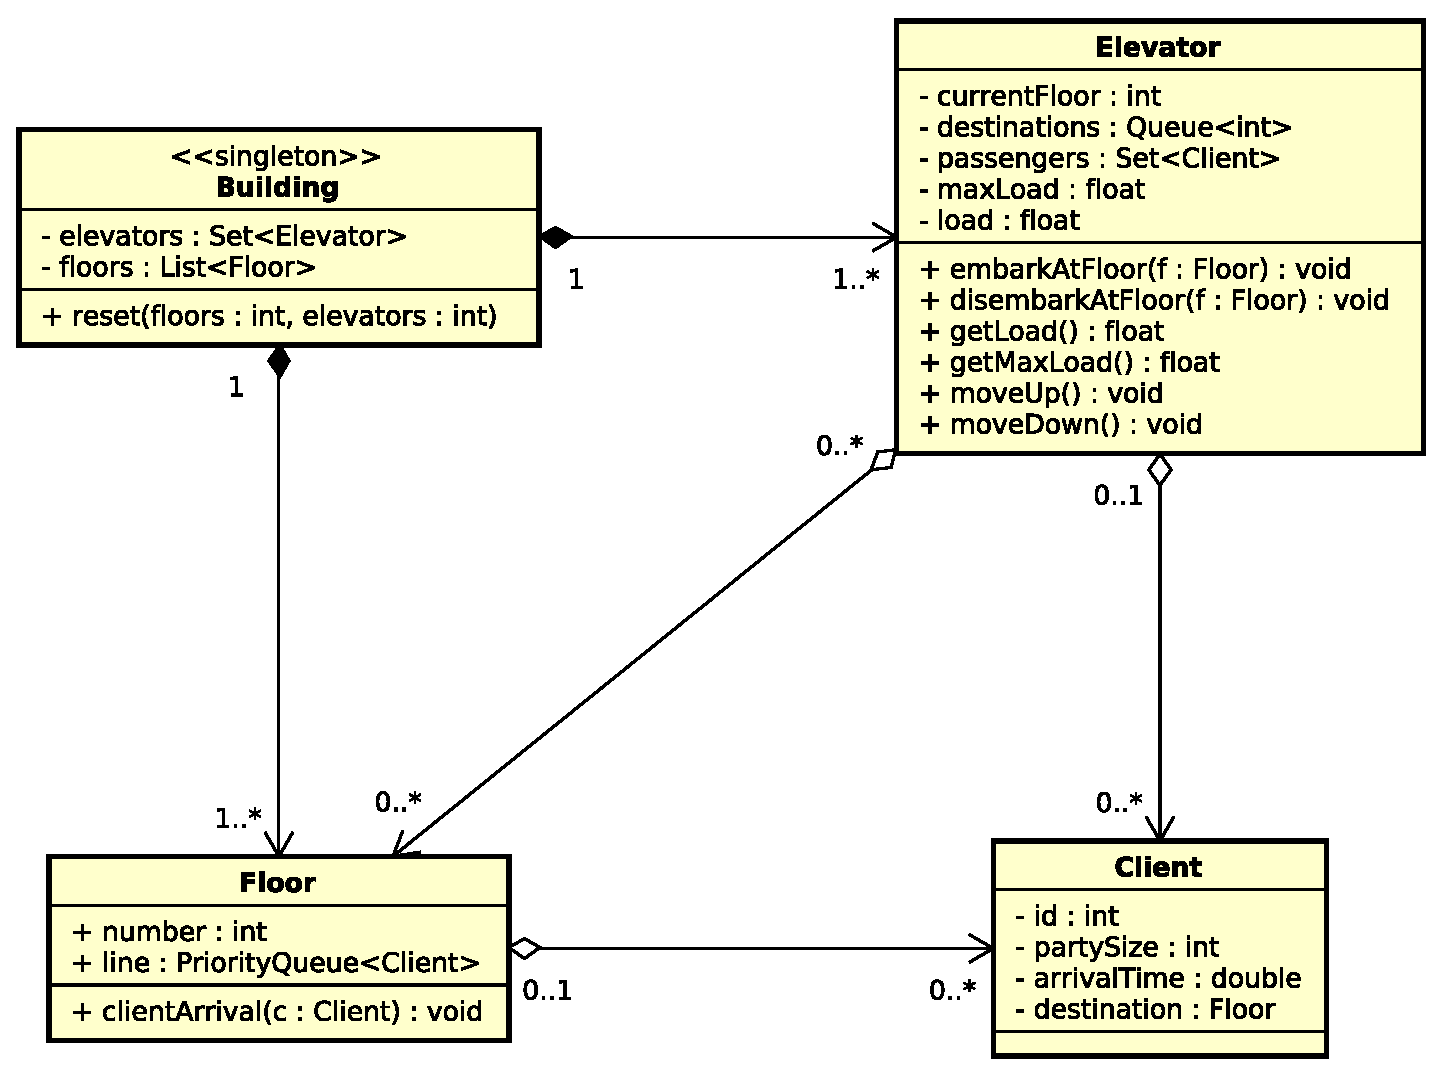
\includegraphics[scale=0.6]{img/state.eps}
  \caption{Diagrama de Classes da Representação do Estado do Sistema}
\label{fig:diagram:system}
\end{figure}

\begin{figure}[htb!]
  \centering
  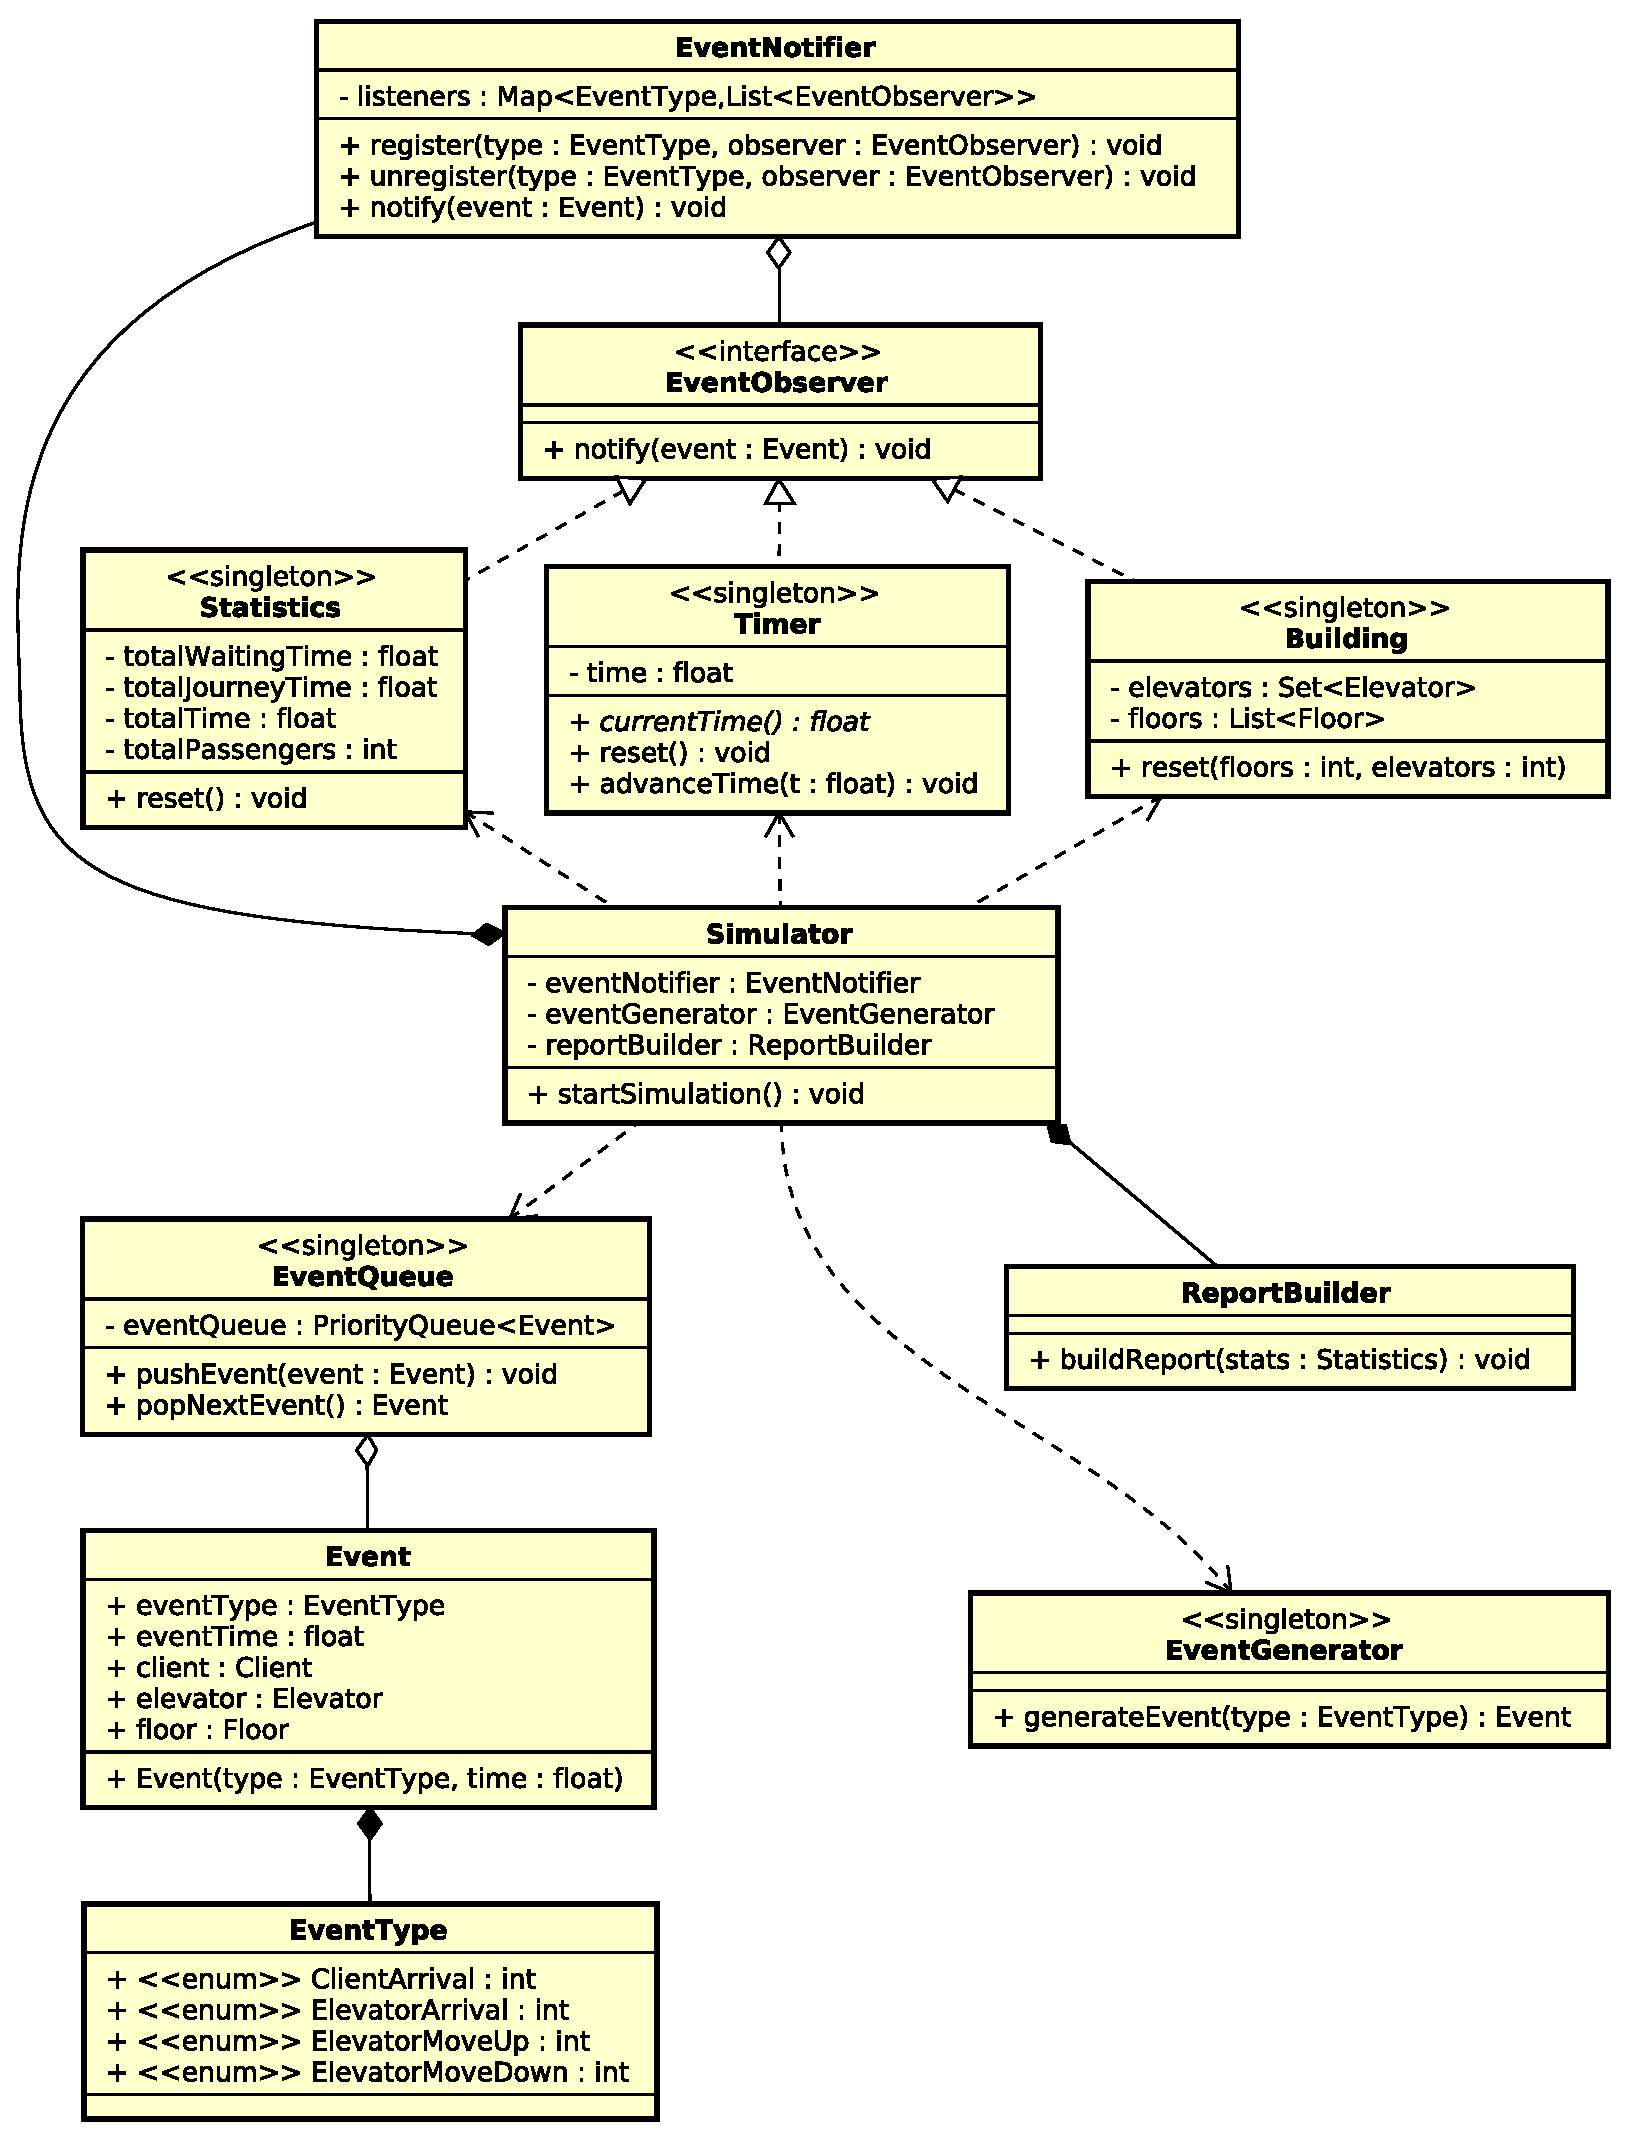
\includegraphics[scale=0.6]{img/simulator.eps}
  \caption{Diagrama de Classes do Simulador}
\label{fig:diagram:simulator}
\end{figure}


\subsection{aaaaaaaa}

Aqui vamos apresentar:

\begin{itemize}
  \item Descrições e diagramas UML dos componentes (classes, algoritmos, etc)
que dão sentido à simulação - ou seja, o modelo do sistema de elevadores
  \item Algoritmos e fluxogramas dos eventos do simulador que causarão
alterações no estado do sistema quais informações desejamos que o simulador
calcule para nós.
\end{itemize}

\section{\label{chap:input}Entrada de Distribuição de Probabilidade}

Aqui vamos apresentar:

\begin{itemize}
\item Conceitos sobre distribuições de probabilidade;
\item Conceitos sobre geração de variáveis aleatórias em ambiente computacional;
\item Descrever o modelo selecionado de processo de chegada de clientes
(passageiros);
\item Algoritmos e fluxogramas dos eventos do simulador que causarão alterações
no estado do sistema.
\end{itemize}